\documentclass[10pt]{article}
\usepackage{graphicx}
\usepackage{amsmath, amsfonts}
\usepackage{float}
\usepackage{multicol}

\title{Support Vector Machine Approach to Breast Cancer Diagnosis}
\author{Colin Samplawski}
\date{Spring 2016}

\begin{document}
\maketitle
\renewcommand{\abstractname}{Preface}
\begin{abstract}
The purpose of this report is to present the work I did on the final project for the course 
CS/Math/Stat/ISyE 525 (Linear Programming Methods) at UW-Madison \cite{525}. I am 
including this as part of my application in order to demonstrate that I have experience 
interacting with research in computer science and writing in a form that is required for 
graduate level work, as well as to display knowledge and experience with a common machine learning technique. All the code used for this project can be found at \texttt{github.com/put\_link\_here}.
\end{abstract}

\section{Introduction}
The data for this project was sourced from the Wisconsin Diagnosis Breast Cancer 
Database which was collected and made available by UW-Madison professors W. Wolberg 
(General Surgery Department), W. Street, and O. Mangasarian (Computer Sciences 
Department) \cite{dataset}. Each member of this data set represents a fine needle aspirate 
taken from a single patient's breast. Each sample was distilled into a 30 dimensional 
real-valued feature vector and given a classifier of either B (benign) or M (malignant) 
\cite{features}. The goal is learn a model which can be used to correctly classify points as benign or malignant with a high degree of accuracy.

\section{Formulation}
The formulation of this problem is based on the material presented in chapter 9 of the 
course textbook written by Michael Ferris (who was also the professor of the course) \cite{textbook}. We have a collection of vectors in $\mathbb{R}^{30}$, and we will divide them into the subsets $\mathcal{M}$ and $\mathcal{B}$ based on classification. Additionally, let $|\mathcal{M}| = m$ and $|\mathcal{B}| = k$. We will construct the following two matrices: $M \in \mathbb{R}^{m \times 30}$ and $B \in \mathbb{R}^{k \times 30}$, where the columns of $M$ are the feature vectors from $\mathcal{M}$, and similarly for $B$ and $\mathcal{B}$. We want to find a linear function $f$, such that $f(x) < 0 \Leftrightarrow x \in B$ and $f(x) > 0 \Leftrightarrow  x \in M$ to the greatest extent possible. Such a function is called a \textit{linear classifier}.

Since we want $f$ to be linear, it will be of the form $f(x)=w^Tx-\gamma$, for some $w \in \mathbb{R}^{30}$ and $\gamma \in \mathbb{R}$. Ideally, there will exist some $w$ and $\gamma$ such that the hyperplane defined by $w$ and $\gamma$ will perfectly divide the set into two regions based on classification, but there could be infinitely such hyperplanes. To account for this, we will use the \textit{maximum-margin method}. 

First note that based on our definition of $f$, if the data is linearly separable, the hyperplane given by $f(x)=0$, that is $w^Tx= \gamma$, will divide the set.  We will then define the \textit{margin} around $f(x)=0$ as the symmetric region bounded by the two parallel hyperplanes given by $w^Tx = \gamma - 1$ and $w^Tx = \gamma + 1$. We want to increase the size of this margin until a point in the set intersects with the one of the planes. So we will now express our desired characteristics of $f$ as follows:  
\begin{equation}
\begin{split}
x \in \mathcal{M} \Leftrightarrow f(x) & = w^Tx- \gamma \geq 1 \\
x \in \mathcal{B}   \Leftrightarrow f(x) & = w^Tx - \gamma \leq -1.
\end{split}
\end{equation}
We can express these conditions for every $x$ using the matrices $M$ and $B$ from above. That is, we are looking for a $w$ and $\gamma$ which satisfy the following system of linear inequalities:
\begin{equation}
\begin{split}
Mw - e \gamma & \geq e\\
-Bw  + e \gamma & \geq e.
\end{split}
\end{equation}
Here $e$ represents a vector of all 1s of proper dimension.

Furthermore, we want to maximize the size of the margin. It can be shown that the distance between the two bounding hyperplanes, i.e. the size of the margin, is given by $\frac{2}{||w||_2}$ \cite{textbook}. Since the $l_2$ norm is self dual, maximizing $\frac{2}{||w||_2}$ is equivalent to minimizing $||w||^2=w^Tw$ \cite{textbook}. Therefore, we can find the best $w$ and $\gamma$ by solving the following quadratic program: 
\begin{equation}
\begin{split}
\min_{w, \gamma} \qquad & \frac{1}{2} w^Tw \\
\text{subject to}  \qquad & Mw - e \gamma \geq e \\
 - & Bw \ + e \gamma  \geq e.
\end{split}
\end{equation}

So far we have assumed that there exists a hyperplane that perfectly splits the data, but in practice it is very unlikely that such a hyperplane will exist. If this is the case then the quadratic program above will be infeasible. To account for this, we will introduce the slack variable $y \in \mathbb{R}^m$ which will account for violation of the constraints associated with $M$. Similarly, we will introduce the slack variable $z \in \mathbb{R}^k$ for the constraints associated with $B$. This gives us the following modified quadratic program:
\begin{equation}
\begin{split}
\min_{w, \gamma,y,z} \qquad & \frac{1}{2} w^Tw + \frac{1}{m}e^Ty + \frac{1}{k}e^Tz\\
\text{subject to}  \qquad & Mw - e \gamma +y \geq e \\
- & Bw \ + e \gamma +z \geq e \\
& \qquad y, z \geq 0.
\end{split}
\end{equation}
Essentially, to ensure that the quadratic program is feasible, we will allow the constraints to be violated by some amount, given by $y$ and $z$. Of course we would like for this violation to as small as possible, so the average of the values of $y$ and $z$ are included in the objective function.  The average is used rather than the raw values so that $y$ and $z$ contribute to the error with the same weight. Solving this program will find the $w$ and $\gamma$ that define the hyperplane which divides the data with the smallest amount of error. Problems of the form given in (4) are often called \textit{support vector machines} (SVM).

\section{Tuning}
In order to avoid over-fitting, a tuning phase was conducted before calculating the final $w$ and $\gamma$. The original dataset was broken into a training, testing, and tuning set, where the training set determines $B$ and $M$. The objective function of (4) was then altered to include a constant tuning factor $\mu$ to give the following new objective function:
\begin{equation}
\min_{w, \gamma,y,z} \qquad  \frac{\mu}{2} w^Tw + \frac{1}{m}e^Ty + \frac{1}{k}e^Tz.
\end{equation}

Tuning then consisted of solving the quadratic program for values of $\mu$ in the series $5e -5,1e-4,1.5e-4,...,5e-4$. The resulting $w$ and $\gamma$ were then used to calculate the classification error on the tuning set. The $\mu$ value that displayed the least amount of error was then used for the rest of the project. I found that a $\mu$ value of $1.5e-4$ resulted in the lowest amount of error.

\section{Results}
An SVM approach proved to be well suited for this particular task. After learning the dividing plane, less than 1\% of training instances were misclassified. Misclassified training instances indicate points that were placed on the wrong side of the dividing plane. Such a low training set error indicts that the dataset is linearly separable in the 30-dimensional space. Furthermore, a testing set error of 7\% was observed. 



In an effort to visualize to the  linear separability of the dataset, the problem was reduced down to two dimensions.  For every pair of features, the quadratic program was recalculated using only the values corresponding to those features. The resulting line was then used to calculate the error in the tuning set. The pair of features that resulted in the lowest error are shown in the following figure.
\begin{figure}
	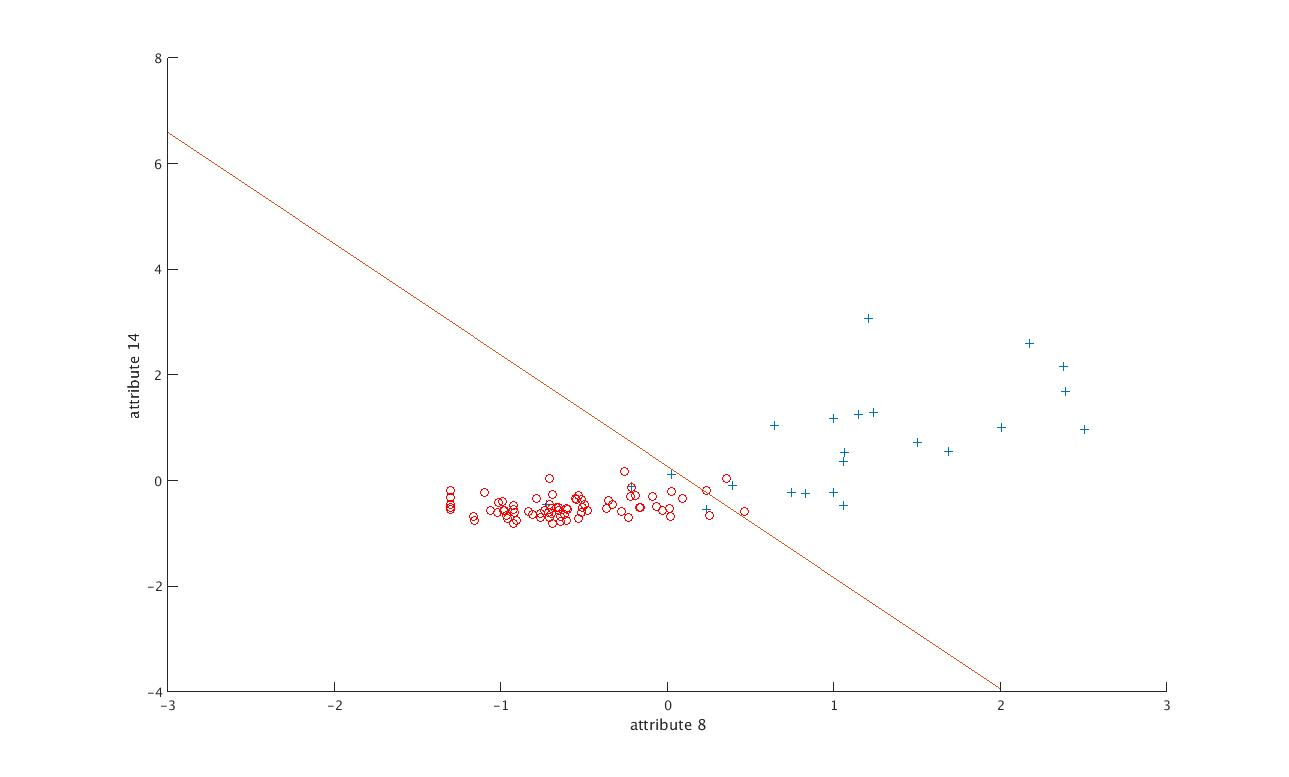
\includegraphics[width=\textwidth]{graph.jpg}
\end{figure}

\pagebreak
\begin{thebibliography}{9}
	\bibitem{525}
	Linear Programming Methods course description,
	\\\texttt{https://www.cs.wisc.edu/courses/525}.  
	
	\bibitem{dataset}
	Breast Cancer Wisconsin (Diagnostic) Data Set,
	\\\texttt{https://archive.ics.uci.edu/ml/datasets/Breast+Cancer+Wisconsin+(Diagnostic)}.
	
	\bibitem{features}
	W.N. Street, W.H. Wolberg and O.L. Mangasarian. Nuclear feature extraction for breast 
	tumor diagnosis. \textit{IS  \& T/SPIE 1993 International Symposium on Electronic 
	Imaging: Science and Technology}, volume 1905, pages 861-870, San Jose, CA, 1993. 
	
	\bibitem{textbook}
	M.C. Ferris, O.L. Mangasarian, S.J. Wright. Linear Programming with MATLAB. \textit{MOS-SIAM Series on Optimization}, 2007.
\end{thebibliography}
\end{document}
